\documentclass[12pt,a4paper]{article}

%% ── Packages ──────────────────────────────────────────────────────────────
\usepackage[a4paper, top=2.5cm, bottom=2.5cm, left=2.5cm, right=2.5cm]{geometry}
\usepackage{amsmath, amssymb, amsthm}
\usepackage{graphicx}
\usepackage{tikz}
\usetikzlibrary{arrows.meta, positioning, shapes.geometric, calc}
\usepackage{pgfplots}
\pgfplotsset{compat=1.18}
\usepackage{booktabs}
\usepackage{array}
\usepackage{enumitem}
\usepackage{hyperref}
\hypersetup{colorlinks=true, linkcolor=black, citecolor=black, urlcolor=black}
\usepackage{fancyhdr}
\usepackage{titlesec}
\usepackage{xcolor}
\usepackage{mdframed}
\usepackage{mathtools}
\usepackage{float}
\usepackage{caption}
\usepackage{subcaption}
\usepackage{setspace}

%% ── Theorem environments ──────────────────────────────────────────────────
\theoremstyle{plain}
\newtheorem{theorem}{Theorem}[section]
\newtheorem{lemma}[theorem]{Lemma}
\newtheorem{corollary}[theorem]{Corollary}
\newtheorem{proposition}[theorem]{Proposition}

\theoremstyle{definition}
\newtheorem{definition}[theorem]{Definition}
\newtheorem{example}[theorem]{Example}
\newtheorem{remark}[theorem]{Remark}

%% ── Framed box for key results ────────────────────────────────────────────
\mdfdefinestyle{keybox}{
  linecolor=black!70,
  linewidth=1pt,
  backgroundcolor=gray!8,
  innertopmargin=8pt,
  innerbottommargin=8pt,
  innerleftmargin=10pt,
  innerrightmargin=10pt,
  skipabove=8pt,
  skipbelow=8pt
}

%% ── Header / footer ──────────────────────────────────────────────────────
\pagestyle{fancy}
\fancyhf{}
\fancyhead[L]{\small Energy Methods for Initial Boundary Value Problems}
\fancyhead[R]{\small Course: Partial Differential Equations}
\fancyfoot[C]{\thepage}
\renewcommand{\headrulewidth}{0.4pt}

%% ── Section formatting ───────────────────────────────────────────────────
\titleformat{\section}{\large\bfseries}{\thesection.}{0.5em}{}[\vspace{-2pt}\rule{\linewidth}{0.4pt}]
\titleformat{\subsection}{\normalsize\bfseries}{\thesubsection.}{0.5em}{}

%% ── Useful macros ─────────────────────────────────────────────────────────
\newcommand{\R}{\mathbb{R}}
\newcommand{\norm}[1]{\left\lVert #1 \right\rVert}
\newcommand{\Ltwo}{L^{2}(0,L)}
\newcommand{\ddt}{\dfrac{d}{dt}}
\newcommand{\pd}[2]{\dfrac{\partial #1}{\partial #2}}

%% ══════════════════════════════════════════════════════════════════════════
\begin{document}

%% ── Title page ────────────────────────────────────────────────────────────
\begin{titlepage}
  \centering
  \vspace*{2cm}
  {\LARGE\bfseries Energy Methods and its Applications to}\\[0.5em]
  {\LARGE\bfseries Uniqueness of Initial Boundary Value Problems}\\[3em]
  {\large Souvik Ghorui \quad (M25MA2008)}\\[1em]
  {\large Course: Partial Differential Equations}\\[4em]
  \begin{abstract}
\noindent
This report presents a self-contained study of the \emph{energy method} for
Initial Boundary Value Problems (IBVPs) in partial differential equations. It mainly focus on proving \emph{uniqueness} of solutions. We first introduce the
general framework of IBVPs and motivate the method by discussing Sharp Hadamard's
notion of well-posedness. The necessary mathematical tools — the $L^2$ norm,
integration by parts, and Gronwall's inequality — are developed carefully.
The energy method is then applied to the heat equation (Dirichlet and Neumann
boundary conditions) and to the wave equation (including the damped case), each
time yielding clean proofs of uniqueness. Two fully worked examples with every
algebraic step are included. The report concludes with a discussion of the
advantages and limitations of the energy approach.
\end{abstract}
\end{titlepage}

%% ── Abstract ──────────────────────────────────────────────────────────────


\vspace{1em}
\tableofcontents
\clearpage

%% ══════════════════════════════════════════════════════════════════════════
\section{Introduction}
\label{sec:intro}

Partial differential equations (PDEs) arise throughout the natural sciences and
engineering: the heat equation models diffusion of temperature, the wave
equation governs vibrating strings and sound, and the Laplace/Poisson equations
describe electrostatic potentials and steady-state temperatures~\cite{Evans, Strauss, John}. In each case,
a physical model is only meaningful if the associated mathematical problem has a
solution that is \emph{unique} and \emph{stable} with respect to the given data.

\begin{figure}[H]
\centering
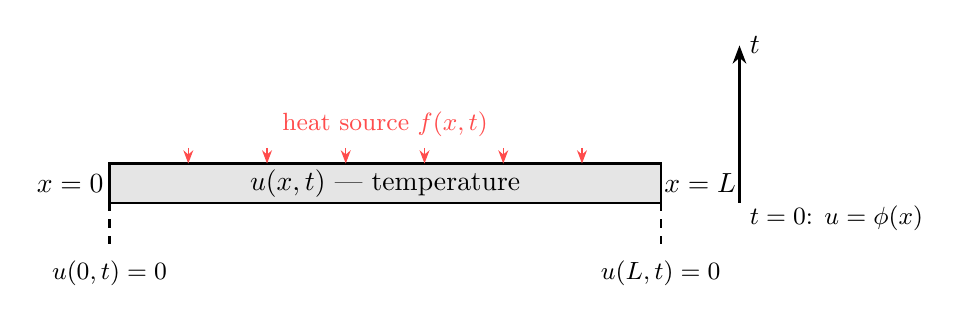
\begin{tikzpicture}[>=Stealth, thick]
  % Draw rod
  \fill[gray!20, draw=black] (0,0) rectangle (7,0.5);
  \node at (-0.5, 0.25) {$x=0$};
  \node at (7.5, 0.25)  {$x=L$};
  % Heat arrows on top
  \foreach \x in {1,2,3,4,5,6}{
    \draw[->, red!70, thin] (\x, 0.7) -- (\x, 0.5);
  }
  \node[red!70] at (3.5, 1.0) {\small heat source $f(x,t)$};
  % Labels inside rod
  \node at (3.5, 0.25) {$u(x,t)$ --- temperature};
  % Boundary conditions
  \draw[dashed] (0,0) -- (0,-0.6);
  \draw[dashed] (7,0) -- (7,-0.6);
  \node[below] at (0, -0.6) {\small $u(0,t)=0$};
  \node[below] at (7, -0.6) {\small $u(L,t)=0$};
  % Time axis
  \draw[->] (8.0, 0.0) -- (8.0, 2.0) node[right] {$t$};
  \node[right] at (8.0, -0.2) {\small $t=0$: $u=\phi(x)$};
\end{tikzpicture}
\caption{A heated rod of length $L$ with Dirichlet (zero-temperature) boundary
  conditions and initial temperature profile $\phi(x)$. The IBVP asks for the
  temperature $u(x,t)$ for all $t>0$.}
\label{fig:rod}
\end{figure}

\subsection{Initial Boundary Value Problems}

An \textbf{Initial Boundary Value Problem (IBVP)} consists of three parts:
\begin{enumerate}[label=(\roman*)]
  \item A PDE that $u(x,t)$ must satisfy in the interior of the domain for $t>0$,
  \item \textbf{Boundary conditions (BCs)} specifying the behaviour of $u$ on
        the boundary of the spatial domain for all $t\geq 0$,
  \item An \textbf{initial condition (IC)} specifying $u$ (and possibly its time
        derivatives) at $t=0$.
\end{enumerate}
In these notes the spatial domain is the interval $(0,L)$, so the general IBVP reads
\begin{align}
  \mathcal{L}[u] &= f(x,t), && x\in(0,L),\; t>0, \label{eq:IBVP-pde}\\
  u(x,0)         &= \phi(x), && x\in[0,L], \label{eq:IBVP-ic}\\
  \text{Boundary conditions} &\text{ at } x=0 \text{ and } x=L, \quad t\geq 0. \label{eq:IBVP-bc}
\end{align}
The most common boundary conditions are:
\begin{itemize}
  \item \textbf{Dirichlet:} $u(0,t)=g_1(t)$, $u(L,t)=g_2(t)$ ,
  \item \textbf{Neumann:} $u_x(0,t)=h_1(t)$, $u_x(L,t)=h_2(t)$ ,
  \item \textbf{Robin/Mixed:} $u_x + \alpha u = 0$ at the boundary .
\end{itemize}

\subsection{Well-Posedness and the Role of Uniqueness}

Hadamard~\cite{hadamard1902} (1902) proposed that a PDE problem is \emph{well-posed} if its
solution: (i) \textbf{exists}, (ii) is \textbf{unique}, and (iii)
\textbf{depends continuously on the data} (stability). Physical models that
fail any of these conditions are unreliable; small measurement errors in the
data could produce arbitrarily large errors in the prediction.

The \emph{energy method} is a technique that addresses the uniqueness and
stability questions \emph{without} needing to find the explicit solution. It
assigns a non-negative scalar quantity $E(t)$ — the \emph{energy} — to the
solution and tracks how $E(t)$ evolves in time. If the energy of the
\emph{difference} of two assumed solutions is shown to be identically zero,
the two solutions must coincide.

%% ══════════════════════════════════════════════════════════════════════════
\section{Mathematical Background}
\label{sec:math}

\subsection{The $L^2$ Norm and Inner Product}

\begin{definition}[$L^2$ Norm]
For a function $f:(0,L)\to\R$, the $L^2$ norm is defined by
\begin{equation}
  \norm{f}^2 \;=\; \norm{f}^2_{L^2(0,L)} \;=\; \int_0^L [f(x)]^2\,dx.
  \label{eq:L2norm}
\end{equation}
\end{definition}

The $L^2$ norm captures the \emph{global} size of $f$ over the whole interval,
in contrast with the maximum norm which only measures the largest pointwise
value. It arises naturally in PDEs because:
\begin{itemize}
  \item For the heat equation, $\int u^2\,dx$ is related to total thermal energy.
  \item For the wave equation, $\int (u_t^2 + u_x^2)\,dx$ represents the sum
        of kinetic and potential energy.
  \item Integration and differentiation interact cleanly via integration by parts~\cite{Kreyszig}.
\end{itemize}

\begin{definition}[$L^2$ Inner Product]
  For two functions $f,g$ on $(0,L)$:
  \begin{equation}
    \langle f,g\rangle \;=\; \int_0^L f(x)\,g(x)\,dx.
    \label{eq:inner}
  \end{equation}
  Note that $\langle f,f\rangle = \norm{f}^2$~\cite{Hardy}.
\end{definition}

\subsection{Integration by Parts}

The single most-used algebraic tool in the energy method is integration by
parts (IBP), which follows directly from the product rule.

\begin{lemma}[Integration by Parts]
  If $f$ and $g$ are differentiable on $[0,L]$, then
  \begin{equation}
    \int_0^L f'(x)\,g(x)\,dx \;=\; \bigl[f(x)g(x)\bigr]_0^L
    \;-\; \int_0^L f(x)\,g'(x)\,dx.
    \label{eq:IBP}
  \end{equation}
\end{lemma}

Setting $f=u_x$ and $g=u$ in \eqref{eq:IBP} yields the key identity
\begin{equation}
  \int_0^L u_{xx}\,u\,dx \;=\; \bigl[u_x\,u\bigr]_0^L \;-\; \int_0^L u_x^2\,dx.
  \label{eq:IBP-key}
\end{equation}
Under \textbf{homogeneous Dirichlet BCs} ($u(0,t)=u(L,t)=0$), the boundary
term vanishes, giving
\begin{equation}
  \int_0^L u_{xx}\,u\,dx \;=\; -\int_0^L u_x^2\,dx \;=\; -\norm{u_x}^2.
  \label{eq:IBP-dirichlet}
\end{equation}
This identity converts the second derivative $u_{xx}$ into the first derivative
$u_x$, which is the key step that makes the energy method work.

\subsection{Differentiation of a Squared Norm}

A simple but fundamental identity governs how the $L^2$ norm of a time-dependent
function evolves:
\begin{equation}
  \ddt \int_0^L [u(x,t)]^2\,dx \;=\; \int_0^L 2\,u\,u_t\,dx \;=\; 2\langle u,u_t\rangle,
  \label{eq:norm-deriv}
\end{equation}
obtained by differentiating under the integral sign. In short,
$\dfrac{d}{dt}\norm{u}^2 = 2\langle u,u_t\rangle$.

\subsection{Gronwall's Inequality}

Gronwall's inequality~\cite{Gronwall} converts a differential or integral inequality into an
explicit upper bound — it is the backbone of every energy estimate.

\begin{theorem}[Gronwall's Inequality — Integral Form]
\label{thm:gronwall}
Let $E(t)\geq 0$ be continuous and satisfy
\begin{equation}
  E(t) \;\leq\; A + B\int_0^t E(s)\,ds, \qquad t\geq 0,
  \label{eq:gronwall-int}
\end{equation}
for constants $A\geq 0$, $B\geq 0$. Then
\begin{equation}
  E(t) \;\leq\; A\,e^{Bt} \qquad \text{for all } t\geq 0.
  \label{eq:gronwall-bound}
\end{equation}
\end{theorem}

\begin{proof}
Define $H(t) = A + B\int_0^t E(s)\,ds$. Then $H(0)=A$, $H'(t)=BE(t)\leq BH(t)$.
Dividing by $H(t)>0$ and integrating from $0$ to $t$:
\[
  \ln H(t) - \ln A \leq Bt \implies H(t)\leq A e^{Bt}.
\]
Since $E(t)\leq H(t)$, the result follows.
\end{proof}

\begin{corollary}[Gronwall's Inequality — Differential Form]
\label{cor:gronwall-diff}
  If $E(t)\geq 0$ is differentiable and $E'(t)\leq C\,E(t)$ for a constant
  $C\in\R$, then
  \begin{equation}
    E(t) \;\leq\; E(0)\,e^{Ct}.
    \label{eq:gronwall-diff}
  \end{equation}
  In particular, if $C\leq 0$, then $E(t)\leq E(0)$ for all $t>0$ — the energy
  does not grow.
\end{corollary}

\begin{remark}
The Poincar\'{e} inequality is also used in energy decay estimates:
\begin{equation}
  \norm{v}^2 \;\leq\; \frac{L^2}{\pi^2}\norm{v_x}^2
  \label{eq:poincare}
\end{equation}
for any $v\in H^1_0(0,L)$~\cite{Brezis} (i.e., $v(0)=v(L)=0$). This allows one to bound the
$L^2$ norm of $v$ by the $L^2$ norm of its derivative.
\end{remark}

%% ══════════════════════════════════════════════════════════════════════════
\section{The Energy Method: Main Theory}
\label{sec:theory}

\subsection{The Energy Functional}

In the energy method, we assign a scalar quantity $E(t)\geq 0$ to the solution
$u(\cdot,t)$, called the \emph{energy functional}. The choice depends on the
equation:
\begin{itemize}
  \item \textbf{Heat equation} (first order in $t$):
        $\displaystyle E(t) = \tfrac{1}{2}\norm{u(\cdot,t)}^2
                             = \tfrac{1}{2}\int_0^L u^2\,dx.$
  \item \textbf{Wave equation} (second order in $t$):
        $\displaystyle E(t) = \tfrac{1}{2}\int_0^L (u_t^2 + c^2 u_x^2)\,dx$,
        which is kinetic $+$ potential energy.
\end{itemize}

\subsection{The Two-Step Strategy}

\begin{mdframed}[style=keybox]
\textbf{Energy Method — Two-Step Strategy}\\[4pt]
\textbf{Step 1 (Energy identity).}
Multiply the PDE by $u$ (for the heat equation) or by $u_t$ (for the wave
equation). Integrate over $x\in(0,L)$, apply IBP, and use the boundary
conditions to eliminate boundary terms. This yields a relation for $E'(t)$.\\[4pt]
\textbf{Step 2 (Gronwall / integration).}
The result from Step 1 is typically an inequality $E'(t)\leq CE(t)+G(t)$.
Apply Gronwall's inequality to obtain an explicit bound on $E(t)$.
\end{mdframed}

\subsection{How Uniqueness Follows}

Suppose $u_1$ and $u_2$ both solve the same IBVP. Define the difference
$w = u_1 - u_2$. By linearity of the PDE operator:
\begin{itemize}
  \item $w$ satisfies the \emph{homogeneous} PDE (source terms cancel),
  \item $w$ satisfies \emph{homogeneous} boundary conditions ($w=0$ on the boundary),
  \item $w$ satisfies \emph{zero} initial condition ($w(x,0)=0$).
\end{itemize}
Apply the energy method to $w$. Define $E_w(t)=\tfrac{1}{2}\norm{w}^2\geq 0$.
If the energy identity gives $E_w'(t)\leq 0$, then since $E_w$ is non-increasing and
\[
  E_w(0) = \tfrac{1}{2}\int_0^L [w(x,0)]^2\,dx = 0,
\]
it follows that $0\leq E_w(t)\leq E_w(0)=0$, i.e.\ $E_w(t)=0$ for all
$t\geq 0$, which forces $w\equiv 0$, hence $u_1=u_2$.

\begin{figure}[H]
\centering
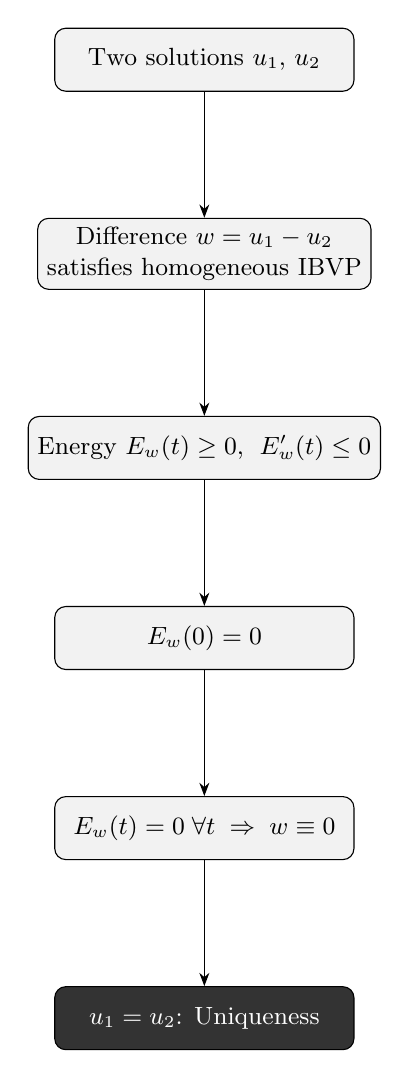
\begin{tikzpicture}[>=Stealth, node distance=1.6cm, every node/.style={font=\small}]
  \node[draw, rounded corners, fill=gray!10, minimum width=3.8cm, minimum height=0.8cm, align=center]
    (A) {Two solutions $u_1,\, u_2$};
  \node[draw, rounded corners, fill=gray!10, minimum width=3.8cm, minimum height=0.8cm, align=center, below=of A]
    (B) {Difference $w = u_1-u_2$\\satisfies homogeneous IBVP};
  \node[draw, rounded corners, fill=gray!10, minimum width=3.8cm, minimum height=0.8cm, align=center, below=of B]
    (C) {Energy $E_w(t)\geq 0$,\; $E_w'(t)\leq 0$};
  \node[draw, rounded corners, fill=gray!10, minimum width=3.8cm, minimum height=0.8cm, align=center, below=of C]
    (D) {$E_w(0)=0$};
  \node[draw, rounded corners, fill=gray!10, minimum width=3.8cm, minimum height=0.8cm, align=center, below=of D]
    (E) {$E_w(t)=0\;\forall t\;\Rightarrow\; w\equiv 0$};
  \node[draw, rounded corners, fill=black!80, text=white, minimum width=3.8cm, minimum height=0.8cm, align=center, below=of E]
    (F) {$u_1 = u_2$: Uniqueness};
  \draw[->] (A)--(B); \draw[->] (B)--(C); \draw[->] (C)--(D);
  \draw[->] (D)--(E); \draw[->] (E)--(F);
\end{tikzpicture}
\caption{Flowchart of the uniqueness argument via the energy method.}
\label{fig:flowchart}
\end{figure}

\subsection{How Stability Follows}

Let $u_1$ solve the IBVP with data $(\phi_1, f_1)$ and $u_2$ with data $(\phi_2,f_2)$.
Set $w=u_1-u_2$ and $F=f_1-f_2$. The energy method applied to $w$ yields a bound of
the form
\[
  E_w(t) \;\leq\; C(T)\Bigl(\norm{\phi_1-\phi_2}^2 + \int_0^t\norm{F(\cdot,s)}^2\,ds\Bigr).
\]
If $\phi_1\to\phi_2$ and $f_1\to f_2$, then $E_w(t)\to 0$ — small changes in data
produce small changes in the solution. This is continuous dependence on data, the
stability aspect of well-posedness.

%% ══════════════════════════════════════════════════════════════════════════
\section{Applications}
\label{sec:applications}

\subsection{Application 1: The Heat Equation (Dirichlet BCs)}

\subsubsection*{Problem Setup}

\begin{mdframed}[style=keybox]
\textbf{Heat Equation IBVP}
\begin{align}
  u_t &= k\,u_{xx} + f(x,t), && x\in(0,L),\; t>0, \label{eq:heat-pde}\\
  u(x,0) &= \phi(x), && x\in[0,L], \label{eq:heat-ic}\\
  u(0,t) &= 0,\quad u(L,t)=0, && t>0. \label{eq:heat-bc}
\end{align}
Here $k>0$ is the thermal diffusivity, $f$ is a heat source/sink, and $\phi$
is the initial temperature profile.
\end{mdframed}

\subsubsection*{Deriving the Energy Identity}

Define $E(t)=\tfrac{1}{2}\norm{u(\cdot,t)}^2$. Differentiating and substituting
the PDE:
\begin{align*}
  E'(t) &= \int_0^L u\,u_t\,dx
          = \int_0^L u\,(k\,u_{xx}+f)\,dx
          = k\int_0^L u\,u_{xx}\,dx + \langle u,f\rangle.
\end{align*}
Applying \eqref{eq:IBP-dirichlet} (boundary terms vanish by \eqref{eq:heat-bc}):
\begin{equation}
  \boxed{E'(t) = -k\norm{u_x}^2 + \langle u,f\rangle.}
  \label{eq:heat-energy}
\end{equation}
The term $-k\norm{u_x}^2\leq 0$ shows that diffusion always \emph{dissipates}
energy; the source term $\langle u,f\rangle$ can add or remove energy.

\subsubsection*{Uniqueness for the Heat Equation}

\begin{theorem}[Uniqueness — Heat Equation]
  \label{thm:heat-unique}
  The IBVP \eqref{eq:heat-pde}--\eqref{eq:heat-bc} has at most one solution.
\end{theorem}

\begin{proof}
Let $u_1,u_2$ solve \eqref{eq:heat-pde}--\eqref{eq:heat-bc} and set $w=u_1-u_2$.
Then $w$ satisfies $w_t = k\,w_{xx}$ with $w(x,0)=0$ and homogeneous Dirichlet BCs.
Define $E_w(t)=\tfrac{1}{2}\norm{w}^2\geq 0$.
By \eqref{eq:heat-energy} with $f=0$:
\[
  E_w'(t) = -k\norm{w_x}^2 \leq 0.
\]
So $E_w$ is non-increasing. Since $E_w(0)=\tfrac{1}{2}\int_0^L[w(x,0)]^2\,dx=0$,
\[
  0 \leq E_w(t) \leq E_w(0) = 0 \implies E_w(t)=0\;\;\forall\, t\geq 0.
\]
Therefore $\int_0^L w^2\,dx=0$, forcing $w\equiv 0$, i.e.\ $u_1=u_2$.
\end{proof}

\subsubsection*{Energy Decay (Homogeneous Case $f=0$)}

Using the Poincar\'{e} inequality \eqref{eq:poincare} in \eqref{eq:heat-energy}
(with $f=0$):
\[
  \norm{u_x}^2 \geq \frac{\pi^2}{L^2}\norm{u}^2 = \frac{2\pi^2}{L^2}E(t).
\]
Hence $E'(t)\leq -\tfrac{2k\pi^2}{L^2}E(t)$, and by Gronwall's inequality:
\begin{equation}
  E(t) \;\leq\; E(0)\,e^{-2k\pi^2 t/L^2}.
  \label{eq:heat-decay}
\end{equation}
The energy decays \emph{exponentially} to zero — the rod eventually cools to
zero temperature, as expected physically.

\begin{figure}[H]
\centering
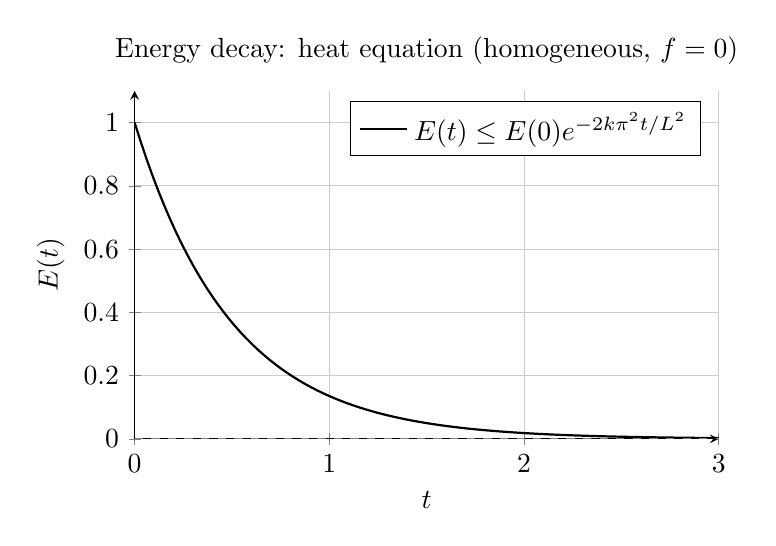
\begin{tikzpicture}
  \begin{axis}[
    width=9cm, height=6cm,
    xlabel={$t$}, ylabel={$E(t)$},
    xmin=0, xmax=3, ymin=0, ymax=1.1,
    xtick={0,1,2,3},
    ytick={0,0.2,0.4,0.6,0.8,1.0},
    axis lines=left,
    grid=both, grid style={line width=0.3pt, gray!40},
    legend pos=north east,
    title={Energy decay: heat equation (homogeneous, $f=0$)}
  ]
    \addplot[black, thick, domain=0:3, samples=100]
      {exp(-2*x)};
    \addlegendentry{$E(t)\leq E(0)e^{-2k\pi^2 t/L^2}$}
    \addplot[dashed, gray, domain=0:3] {0};
  \end{axis}
\end{tikzpicture}
\caption{Exponential decay of the energy $E(t)$ for the homogeneous heat equation
  with Dirichlet boundary conditions. The constant in the exponent depends on $k$
  and $L$.}
\label{fig:heat-decay}
\end{figure}

\subsection{Application 2: Heat Equation with Neumann Boundary Conditions}

\begin{mdframed}[style=keybox]
\textbf{Neumann IBVP (Insulated Ends)}
\begin{align}
  u_t &= k\,u_{xx}, && x\in(0,L),\; t>0,\\
  u(x,0) &= \phi(x), && x\in[0,L],\\
  u_x(0,t) &= 0,\quad u_x(L,t)=0, && t>0.
\end{align}
\end{mdframed}
These BCs model a rod whose ends are thermally insulated (no heat flux).
Integration by parts now gives
\[
  \int_0^L u\,u_{xx}\,dx = \bigl[u\,u_x\bigr]_0^L - \norm{u_x}^2
  = u(L)u_x(L) - u(0)u_x(0) - \norm{u_x}^2 = -\norm{u_x}^2,
\]
since $u_x(0,t)=u_x(L,t)=0$. The energy identity is the same as
\eqref{eq:heat-energy} (with $f=0$), so uniqueness follows by the same argument.
In addition, integrating the PDE over $(0,L)$ shows that the total heat is
conserved:
\[
  \ddt\int_0^L u\,dx = k\int_0^L u_{xx}\,dx = k\bigl[u_x\bigr]_0^L = 0.
\]

\subsection{Application 3: The Wave Equation}

\subsubsection*{Problem Setup}

\begin{mdframed}[style=keybox]
\textbf{Wave Equation IBVP}
\begin{align}
  u_{tt} &= c^2 u_{xx} + f(x,t), && x\in(0,L),\; t>0, \label{eq:wave-pde}\\
  u(x,0) &= \phi(x),\quad u_t(x,0)=\psi(x), && x\in[0,L], \label{eq:wave-ic}\\
  u(0,t) &= 0,\quad u(L,t)=0, && t>0. \label{eq:wave-bc}
\end{align}
Here $c>0$ is the wave speed, $\phi$ is the initial displacement, and $\psi$
is the initial velocity.
\end{mdframed}

\subsubsection*{Choosing the Right Energy}

For a second-order-in-time equation we include both kinetic and potential energy:
\begin{equation}
  E(t) = \frac{1}{2}\int_0^L \bigl(u_t^2 + c^2 u_x^2\bigr)\,dx.
  \label{eq:wave-energy}
\end{equation}
Note $E(t)\geq 0$ and $E(t)=0 \iff u_t\equiv 0$ and $u_x\equiv 0$, which with
the BCs implies $u\equiv 0$.

\subsubsection*{Deriving the Energy Identity}

Multiply the PDE \eqref{eq:wave-pde} by $u_t$ and integrate over $(0,L)$:
\begin{align*}
  E'(t)
  &= \int_0^L (u_t u_{tt} + c^2 u_x u_{xt})\,dx.
\end{align*}
Apply IBP to the term $c^2\int_0^L u_x u_{xt}\,dx$ (boundary terms vanish since
$u_t(0,t)=u_t(L,t)=0$ from the Dirichlet BCs):
\[
  c^2\int_0^L u_x u_{xt}\,dx = -c^2\int_0^L u_{xx} u_t\,dx.
\]
Hence
\[
  E'(t) = \int_0^L u_t\,(u_{tt}-c^2 u_{xx})\,dx = \int_0^L u_t\,f\,dx,
\]
where we used $u_{tt}-c^2 u_{xx}=f$. This gives the energy identity:
\begin{equation}
  \boxed{E'(t) = \langle u_t, f\rangle.}
  \label{eq:wave-energy-id}
\end{equation}
When $f=0$: $E'(t)=0$, so $E(t)=E(0)$ — the wave equation \emph{conserves}
energy, in sharp contrast to the heat equation.

\subsubsection*{Uniqueness for the Wave Equation}

\begin{theorem}[Uniqueness — Wave Equation]
  \label{thm:wave-unique}
  The IBVP \eqref{eq:wave-pde}--\eqref{eq:wave-bc} has at most one solution.
\end{theorem}

\begin{proof}
Let $u_1,u_2$ solve the IBVP and set $w=u_1-u_2$. Then $w$ satisfies
$w_{tt}=c^2 w_{xx}$ with $w(x,0)=0$, $w_t(x,0)=0$, and homogeneous BCs.
Define $E_w(t)=\tfrac{1}{2}\int_0^L(w_t^2+c^2 w_x^2)\,dx\geq 0$.
By \eqref{eq:wave-energy-id} with $f=0$: $E_w'(t)=0$, so $E_w(t)=E_w(0)$ for all $t$.
Computing $E_w(0)$:
\[
  E_w(0) = \frac{1}{2}\int_0^L\bigl([w_t(x,0)]^2 + c^2[w_x(x,0)]^2\bigr)\,dx = 0,
\]
since $w_t(x,0)=0$ and $w_x(x,0)=\tfrac{\partial}{\partial x}[w(x,0)]=0$.
Therefore $E_w(t)=0$, forcing $w_t\equiv 0$ and $w_x\equiv 0$.
So $w$ is constant in $x$ and $t$; since $w(x,0)=0$, we get $w\equiv 0$ $\implies u_1 = u_2$.
\end{proof}

%% ══════════════════════════════════════════════════════════════════════════
\section{Worked Examples}
\label{sec:examples}

\subsection{Example 1: Heat Equation}

\begin{example}
\label{ex:heat-reaction}
Consider the IBVP on $(0,\pi)$:
\begin{align*}
  u_t &= u_{xx} + u, \quad x\in(0,\pi),\; t>0,\\
  u(x,0) &= \sin x, \quad x\in[0,\pi],\\
  u(0,t) &= 0, \quad u(\pi,t) = 0.
\end{align*}
\textbf{(a)} Find the energy equation.
\textbf{(b)} Determine whether the energy grows or decays.
\textbf{(c)} Prove uniqueness using the energy method.
\end{example}

\textbf{Solution.}

\textbf{Part (a).} Take $k=1$, $f=u$, $L=\pi$. Define $E(t)=\tfrac{1}{2}\norm{u}^2$.
Applying \eqref{eq:heat-energy} with $f=u$:
\[
  E'(t) = -\norm{u_x}^2 + \langle u,u\rangle = -\norm{u_x}^2 + \norm{u}^2.
\]

\textbf{Part (b).} By the Poincar\'{e} inequality \eqref{eq:poincare} with $L=\pi$:
\[
  \norm{u_x}^2 \geq \frac{\pi^2}{\pi^2}\norm{u}^2 = \norm{u}^2.
\]
Therefore:
\[
  E'(t) = -\norm{u_x}^2 + \norm{u}^2 \leq -\norm{u}^2 + \norm{u}^2 = 0.
\]
Hence $E'(t)\leq 0$: the energy is \emph{non-increasing}. One can verify with the
exact solution $u(x,t)=\sin x$ (since $(\sin x)_t=0=(\sin x)_{xx}+\sin x$): the
energy is constant $E(t)=\pi/4$, consistent with $E'(t)\leq 0$.

\textbf{Part (c).} For uniqueness, let $w=u_1-u_2$ satisfy $w_t=w_{xx}+w$,
$w(x,0)=0$, homogeneous BCs. From Part (b), $E_w'(t)\leq 0$ and $E_w(0)=0$,
so $E_w(t)=0$ and $w\equiv 0$. Uniqueness follows.

\subsection{Example 2:Damped Wave Equation}

\begin{example}
\label{ex:damped-wave}
Consider the damped wave equation:
\begin{align*}
  u_{tt} + 2\gamma u_t &= c^2 u_{xx}, \quad x\in(0,L),\; t>0,\\
  u(x,0) &= \phi(x),\quad u_t(x,0)=\psi(x),\\
  u(0,t) &= 0,\quad u(L,t)=0.
\end{align*}
Here $\gamma>0$ is the damping coefficient.
\textbf{(a)} Derive the energy equation.
\textbf{(b)} Show the energy is non-increasing.
\textbf{(c)} Prove uniqueness.
\end{example}

\textbf{Solution.}

\textbf{Part (a).} Use $E(t)=\tfrac{1}{2}\int_0^L(u_t^2+c^2 u_x^2)\,dx$. Multiplying
the PDE by $u_t$ and integrating (same IBP steps as Section~\ref{sec:applications}):
\[
  E'(t) = \int_0^L u_t\,(u_{tt}-c^2 u_{xx})\,dx.
\]
The PDE gives $u_{tt}-c^2 u_{xx}=-2\gamma u_t$. Therefore:
\begin{equation}
  E'(t) = -2\gamma\norm{u_t}^2 \leq 0.
  \label{eq:damped-energy}
\end{equation}

\textbf{Part (b).} Since $\gamma>0$ and $\norm{u_t}^2\geq 0$, we have $E'(t)\leq 0$,
so $E(t)\leq E(0)$ for all $t$. The damping term dissipates energy — the string
gradually comes to rest.

\textbf{Part (c).} For uniqueness, let $w=u_1-u_2$ satisfy the homogeneous damped
wave equation with zero initial data. Then $E_w'(t)=-2\gamma\norm{w_t}^2\leq 0$ and
$E_w(0)=0$, so $E_w(t)=0$ and $w\equiv 0$. \qed

\begin{figure}[H]
\centering
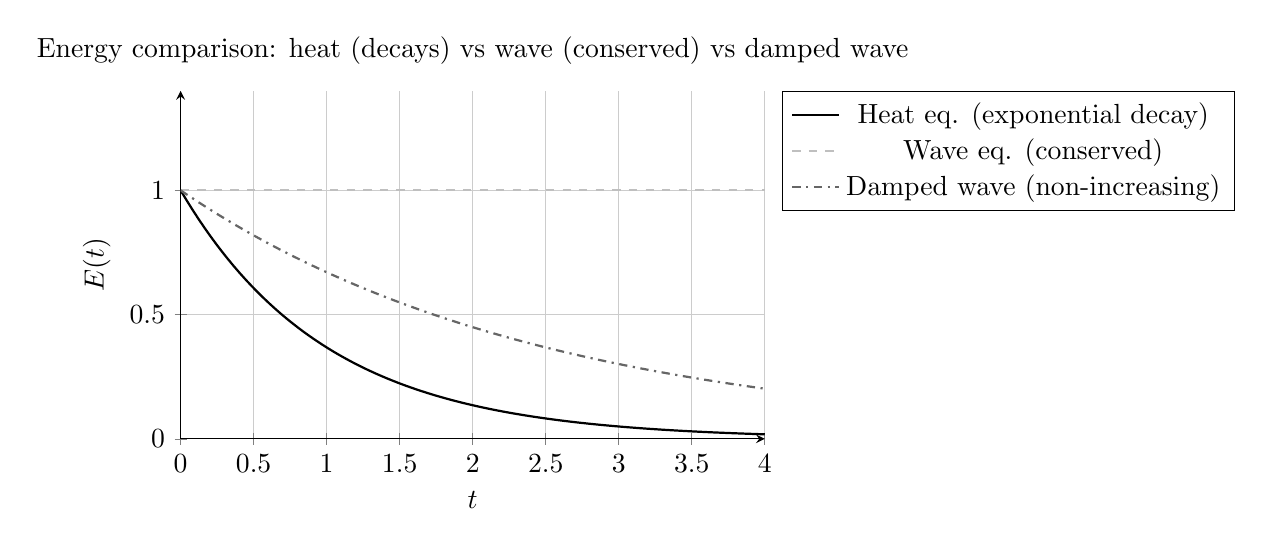
\begin{tikzpicture}
  \begin{axis}[
    width=9cm, height=6cm,
    xlabel={$t$}, ylabel={$E(t)$},
    xmin=0, xmax=4, ymin=0, ymax=1.4,
    axis lines=left,
    grid=both, grid style={line width=0.3pt, gray!40},
    legend pos=outer north east,
    title={Energy comparison: heat (decays) vs wave (conserved) vs damped wave}
  ]
    \addplot[black, thick, domain=0:4, samples=100] {exp(-x)};
    \addlegendentry{Heat eq. (exponential decay)}
    \addplot[gray!50, thick, dashed, domain=0:4] {1.0};
    \addlegendentry{Wave eq. (conserved)}
    \addplot[black!60, thick, dashdotted, domain=0:4, samples=100] {exp(-0.4*x)};
    \addlegendentry{Damped wave (non-increasing)}
  \end{axis}
\end{tikzpicture}
\caption{Qualitative energy behaviour for the three equations studied.
  The heat equation dissipates energy exponentially; the undamped wave equation
  conserves it; the damped wave equation dissipates it at a rate controlled by
  the damping coefficient $\gamma$.}
\label{fig:energy-comparison}
\end{figure}

%% ══════════════════════════════════════════════════════════════════════════
\section{Discussion}
\label{sec:discussion}

\subsection{Strengths of the Energy Method}

\begin{enumerate}[label=\textbf{\arabic*.}]
  \item \textbf{No explicit solution required.}
        The method establishes uniqueness purely from the structure of the equation
        and the boundary conditions, without ever computing $u(x,t)$ in closed form.
  \item \textbf{Flexibility.}
        The same two-step strategy (derive an energy identity, apply Gronwall) works
        for linear and many nonlinear PDEs, in one or more space dimensions.
  \item \textbf{Quantitative stability.}
        The energy estimate directly yields an explicit bound on how much the
        solution can change when the data changes — a quantitative stability
        result.
  \item \textbf{Physical insight.}
        The choice of energy functional mirrors physical energy, giving the
        mathematics a direct connection to the underlying physics (thermal energy,
        mechanical energy, etc.).
\end{enumerate}

\subsection{Limitations}

\begin{enumerate}[label=\textbf{\arabic*.}]
  \item \textbf{Only $L^2$ information.}
        Energy estimates control the $L^2$ norm of the solution. They do not
        directly give pointwise information (e.g.\ the maximum of $u$).
  \item \textbf{Linear problems.}
        For nonlinear PDEs, deriving a useful energy identity can be significantly
        harder. Additional terms may appear that cannot be absorbed into the energy.
  \item \textbf{Does not prove existence.}
        Uniqueness and stability do not imply that a solution exists; existence
        must be established separately (e.g.\ by constructive methods or functional
        analysis).
\end{enumerate}


%% ══════════════════════════════════════════════════════════════════════════
\section{Conclusion}
\label{sec:conclusion}

The energy method is a powerful, general technique for establishing the
uniqueness and stability of solutions to Initial Boundary Value Problems for
PDEs. The central idea is elegant: instead of finding the solution explicitly,
one assigns an energy functional $E(t)\geq 0$ to the solution, derives an
ordinary differential inequality for $E(t)$, and applies Gronwall's inequality
to control the growth of $E$.

For the heat equation, the energy decays — diffusion is inherently dissipative.
For the wave equation, the energy is conserved in the absence of forcing —
reflecting the physical conservation of mechanical energy. Damping introduces
dissipation and drives the energy to zero. In all three cases, the same
two-step strategy yields clean, rigorous proofs of uniqueness.

The key mathematical tools required are the $L^2$ norm, integration by parts
(which converts second derivatives to first derivatives and eliminates boundary
terms), and Gronwall's inequality (which solves the resulting ODE inequality).
The Poincar\'{e} inequality further allows one to obtain exponential decay rates
for the heat equation.

The energy method does not require knowing the explicit solution, making it
applicable even when closed-form solutions are unavailable. Together with the
maximum principle~\cite{Protter} and existence theories, it forms one of the three pillars of
the analysis of PDEs.

%% ── AI Assistance Disclosure ─────────────────────────────────────────────
\subsection*{AI Assistance Disclosure}

\begin{itemize}
    \item \textbf{AI Tool:} Claude (Anthropic) \\
    \textbf{Prompt:} Write me a Latex code to generate the sample report and write the hand written notes and mathematical contents in the generated file. \\
    \textbf{Usage:} Used to assist in structuring the report and formatting the \LaTeX{} source. All mathematical content, derivations, and proofs were drawn from the provided study notes and standard PDE references, and were verified independently.
    
    \medskip % Adds a little vertical space between items

    \item \textbf{AI Tool:} Gemini (Google) \\
    \textbf{Prompt:} write me a code using html, css and javascript to make a interactive environment to show how a reaction diffusion model (pde) works in real life. make it mathematically correct. the equation is $u_t = k u_{xx} + r u$. \\
    \textbf{Usage:} Used to generate a functional HTML/JS environment that numerically solves a linear reaction-diffusion PDE using finite difference spatial discretization and Euler time integration.
    
    \medskip % Adds a little vertical space between items

    \item \textbf{AI Tool:} Gemini (Google) \\
    \textbf{Prompt:} write me a code using html, css and javascript to make a interactive environment to show how a damped wave model (pde) works in real life. make it mathematically correct. the equation is $u_{tt} + 2 \gamma u_t = c^2 u_{xx}$. \\
    \textbf{Usage:} Used to write an HTML, CSS, and JavaScript script that builds an interactive, mathematically accurate simulation of a damped wave PDE model.
\end{itemize}

%% ══════════════════════════════════════════════════════════════════════════
\begin{thebibliography}{9}

\bibitem{Evans}
L.~C.~Evans, \textit{Partial Differential Equations}, 2nd ed.
American Mathematical Society, Graduate Studies in Mathematics, Vol.~19, 2010.

\bibitem{Strauss}
W.~A.~Strauss, \textit{Partial Differential Equations: An Introduction}, 2nd ed.
Wiley, 2008.

\bibitem{hadamard1902}
J.~Hadamard,
\emph{Sur les problemes aux derivees partielles et leur signification physique},
Princeton university Bulletin, 1902.

\bibitem{Kreyszig} 
E. Kreyszig. \emph{Introductory Functional Analysis with Applications}. John Wiley \& Sons, 1989.

\bibitem{Gronwall} T. H. Gronwall. \emph{Note on the derivatives with respect to a parameter of the solutions of a system of differential equations}. Annals of Mathematics 20(4):292-296 (1919).

\bibitem{Hardy}
Hardy, G. H., Littlewood, J. E., \& polya, G. \emph{Inequalities,} Cambridge University Press.

\bibitem{Brezis}
Brezis, H, \emph{Functional Analysis, Sobolev Spaces and Partial Differentian Equations, Springer.} 2010.

\bibitem{John}
F.~John, \textit{Partial Differential Equations}, 4th ed.
Springer, Applied Mathematical Sciences, Vol.~1, 1982.

\bibitem{Protter}
Protter, M. H., \& Weinberger, H. F., \emph{Maximum Principles in Differential Equations,} Springer, 1984.

\end{thebibliography}

\end{document}